\documentclass[a4paper,11pt,reqno]{report}

% --------------------------------------------------------
% Packages
% --------------------------------------------------------
\usepackage{mathtools,graphicx}
\usepackage[colorlinks=true, allcolors=blue]{hyperref}
\usepackage[utf8]{inputenc}
\usepackage{amsmath,amsfonts,amssymb,amsthm,mathrsfs,bm}
\usepackage[margin=20mm]{geometry}
\usepackage{setspace}
\usepackage[table,xcdraw,svgnames]{xcolor}
\usepackage{float} % 支持图片浮点嵌入 e.g.,\begin{figure}[H]
\usepackage{subcaption} % 支持多图
\usepackage{cite}
\usepackage{listings}
\usepackage{tabularx}
\usepackage{url} % bibTex支持引用网页

% --------------------------------------------------------
% Custom Colours
% --------------------------------------------------------
\renewcommand{\baselinestretch}{1.5}    % 1.5-line spacing
\renewcommand{\rmdefault}{phv} % Arial
\renewcommand{\sfdefault}{phv} % Arial
\renewcommand\thesection{\arabic {section}} % Section numbers start from 1
\renewcommand{\bibname}{References}
\newcommand{\HRule}{\rule{\linewidth}{0.5mm}}
\DeclareUnicodeCharacter{2212}{-}
\renewcommand{\thefootnote}{**} 
% --------------------------------------------------------
% Custom Code - R
% --------------------------------------------------------
\lstset{language=R,
    basicstyle=\small\ttfamily,
    stringstyle=\color{DarkGreen},
    otherkeywords={0,1,2,3,4,5,6,7,8,9},
    morekeywords={TRUE,FALSE},
    deletekeywords={data,frame,length,as,character},
    % keywordstyle=\color{blue},
    commentstyle=\color{DarkGreen},
    showstringspaces=false,%without this there will be a symbol in the places where there is a space
    numbers=left,%
    numberstyle={\tiny \color{black}},% size of the numbers
    numbersep=-5pt, % this defines how far the numbers are from the text
}

% --------------------------------------------------------
% Open Page
% --------------------------------------------------------
\begin{document}

\begin{titlepage}

    \begin{center}
    % \begin{figure}[t]
    %     \centering
    %     \includegraphics[width=0.7\textwidth]{figures/QUB_logo.png}
    %     \label{Fig.QUB_logo}
    % \end{figure}
    
    % Upper part of the page
    
    % \textsc{\LARGE Queen's University Belfast}\\[1.5cm]
    
    % \textsc{\Large ELE8096 Wireless Sensor Systems}\\[0.5cm]
    
    
    % Title
    \HRule \\[1cm]
    { \huge \bfseries Coursework 2}\\[0.5cm]
    { \huge \bfseries Linear Regression}\\[0.5cm]
    \HRule \\[1.5cm]
    
    %Author and supervisor
    % \begin{minipage}{0.4\textwidth}
    %     \begin{flushleft} \large
    %         \emph{Author:}\\
    %         Zichi Zhang\\
    %         Muzixiang Xiao\\
    %         Jiyu Zou\\
    %         Yuhang Zhang\\
    %         Chuao Zheng\\
    %         Yujie Yang
    %     \end{flushleft}
    % \end{minipage}
    % \begin{minipage}{0.4\textwidth}
    %     \begin{flushright} \large
    %         \emph{Student Number:} \\
    %         40299571\\
    %         40344034\\
    %         40344452\\
    %         40319754\\
    %         40336028\\
    %         40348355
    %     \end{flushright}
    % \end{minipage}\vspace{1cm}
    % \begin{minipage}{0.4\textwidth}
    %     \begin{flushleft} \large
    %         \emph{Supervisor:}\\
    %         Dr.~E. Garcia-Palacios
    %     \end{flushleft}
    % \end{minipage}
    % \begin{minipage}{0.4\textwidth}
    %     \begin{flushright} \large
    %         \emph{Module Number:} \\
    %         ELE8096
    %     \end{flushright}
    % \end{minipage}
    \begin{table}[H]
        \centering
        \begin{tabularx}{\textwidth}{llX}
            \emph{Author:} & \emph{Student Number:} & \emph{Team member roles:} \\
            Zichi Zhang & 40299571 & Working on building multi variable regression models.\\
            Muzixiang Xiao & 40344034 & Looking at data pre-processing and basic statistics: boxplot in R.\\
            Jiyu Zou & 40344452 & Looking at further statistics (correlation among variables, presenting correlation matrixes, distributions and histograms).\\
            Yuhang Zhang & 40319754 & Working on building multi variable regression models.\\
            Chuao Zheng & 40336028 & Looking at data pre-processing and basic statistics: boxplot in R.\\
            Yujie Yang & 40348355 &  Looking at further statistics (correlation among variables, presenting correlation matrixes, distributions and histograms).\\
            &&\\
            \emph{Supervisor:}&&\emph{Module Number:} \\
            Dr.~E. Garcia-Palacios && ELE8096
        \end{tabularx}
        % \caption{Caption}
        % \label{tab:my_label}
    \end{table}

    \vfill
    
    % Bottom of the page
    {\large \today}
    
    \end{center}
    
    \end{titlepage}

% --------------------------------------------------------
% Abstract
% --------------------------------------------------------
\begin{abstract}
    Data analysing and prediction has become one of the most useful tools recently, 
    trend of data could be deduced by applying linear regression. 
    For group project, it aims to analyse data of concentration of pollutants (NO3, PM2.5, O3) in Belfast for each hour, 
    besides, the relationship between each pollutant and other parameters like humidity and temperature should be revealed after analysing data. R is used for data processing and trend prediction which will be discussed on following paragraphs. 
    The distribution of each pollutant will be analysed firstly in section 2. 
    In section 3, the correlation between each pollutant will be discussed. 
    After that, prediction of trend of data using linear regression with R is presented in section 4, we build three models to compare the performance of models. In section 5, the model performance and the results are discussed. And find that multi variables regression as the model is better. Finally the conclusion will be made at the end of the report. 
\end{abstract}

% --------------------------------------------------------
% Section 1: Introduction
% --------------------------------------------------------
\section{Introduction}
\label{sec:Introduction}
As one of the most developed countries, UK spends a lot of energy per year, such as coal and natural gas. These energy guarantee the daily life of the city which also lead to air pollution. To ensure that people have a healthy environment, the detection of air quality is becoming more and more important, and the analysis of air quality data is the most critical part of it.
\\
\\
Linear regression is a popular analytical method in the field of data analysis. It is an attempt to model the relationship between two variables by fitting a linear equation to observed data, where one variable is an explanatory variable and the other is a dependent variable. The advantage of regression analysis is that it can allow you to essentially crunch the data to help to make better decisions for currently and future.
\\
\\
The regression method of forecasting means investigating on the relationships between data points, which help to predict data in the short and long term. Also, it allows people to understand how different variables impact on the trend of data predicted.
\\
\\
In this paper, a data set containing air quality is analyzed using linear regression. This data was collected in Belfast and it contains concentration of PM2.5, NO2, 03, and related temperature and humidity which collected via a multi-sensor platform (sensor system) each hour. .
\newpage

% --------------------------------------------------------
% Section 2: basic statistics
% --------------------------------------------------------
\section{basic statistics}
\label{sec:basic statistics}
% \subsection{PM2.5}
\begin{figure}[H]
    \centering
    \vspace{-0.35cm}
    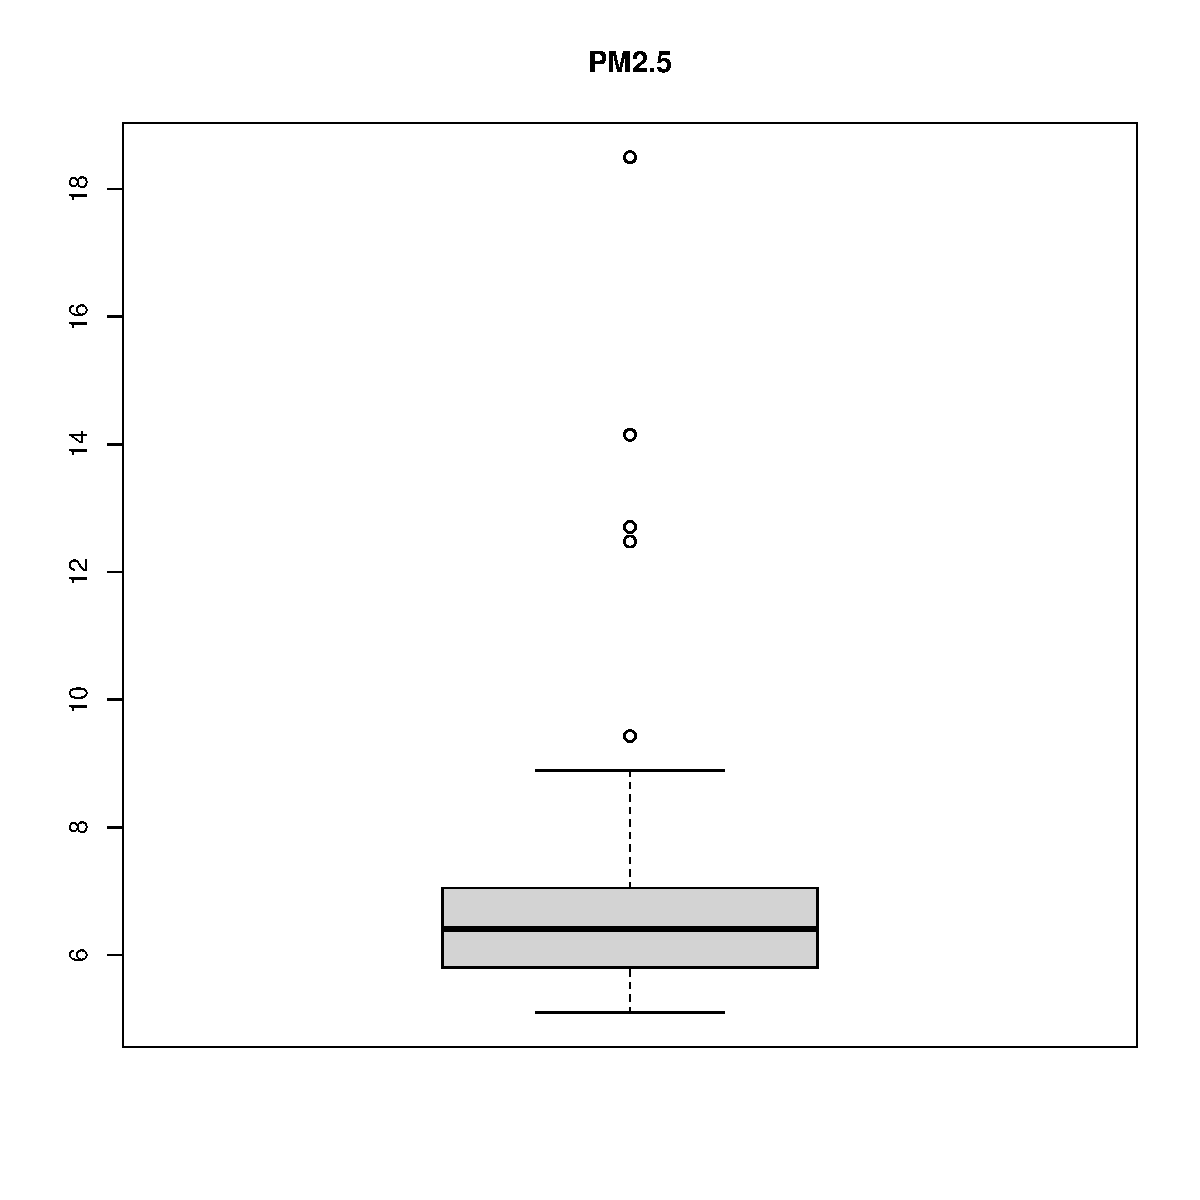
\includegraphics[width=0.4\linewidth]{figures/PM25_box.pdf}
    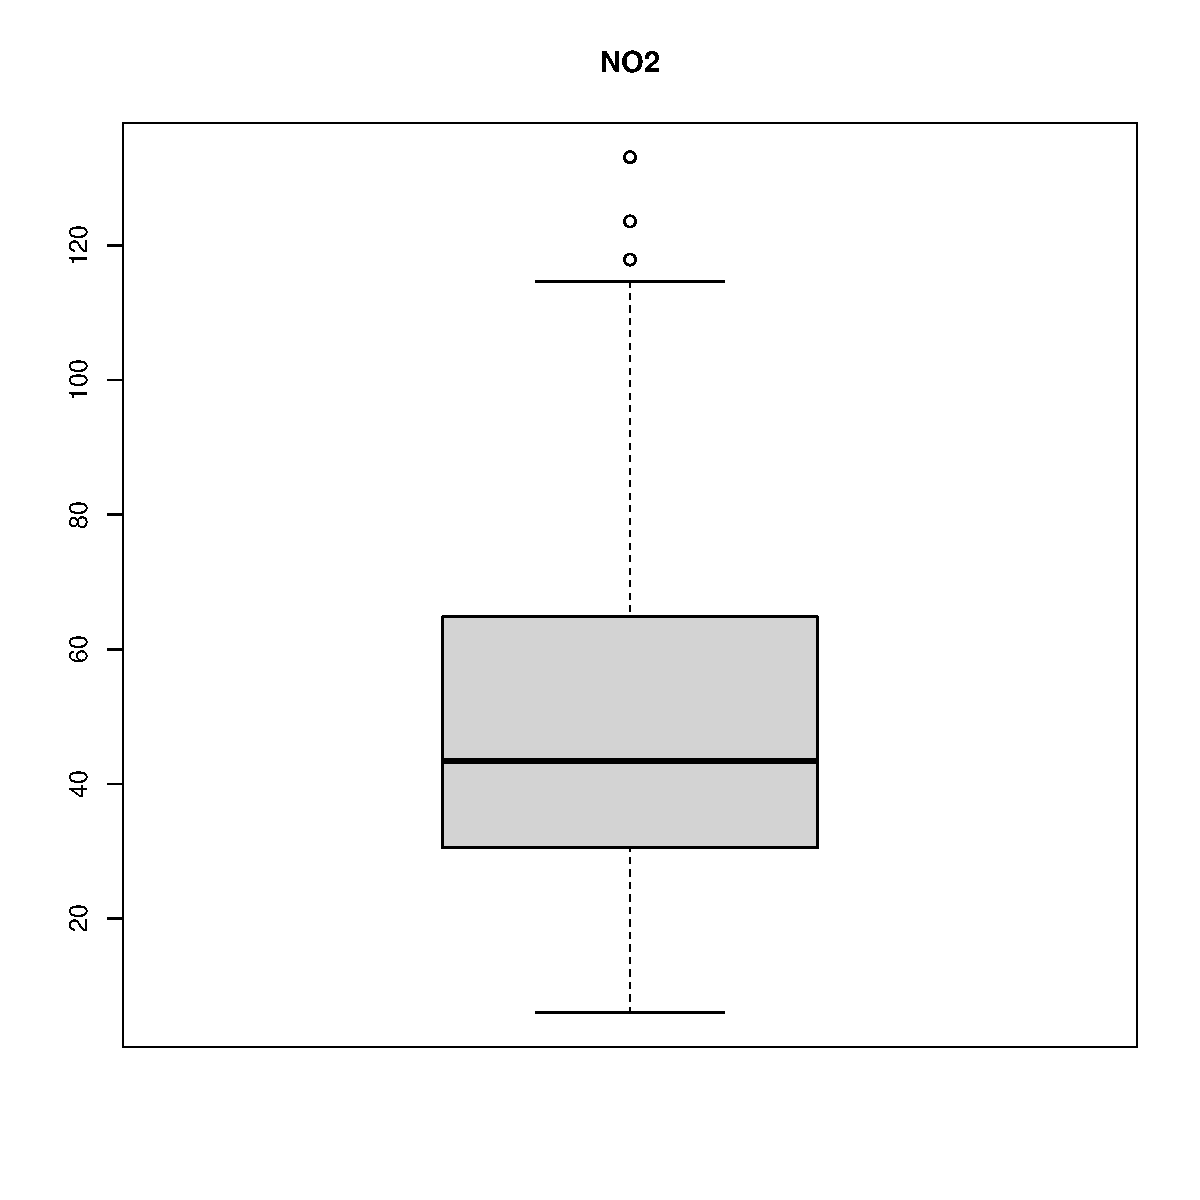
\includegraphics[width=0.4\linewidth]{figures/NO2_box.pdf}
    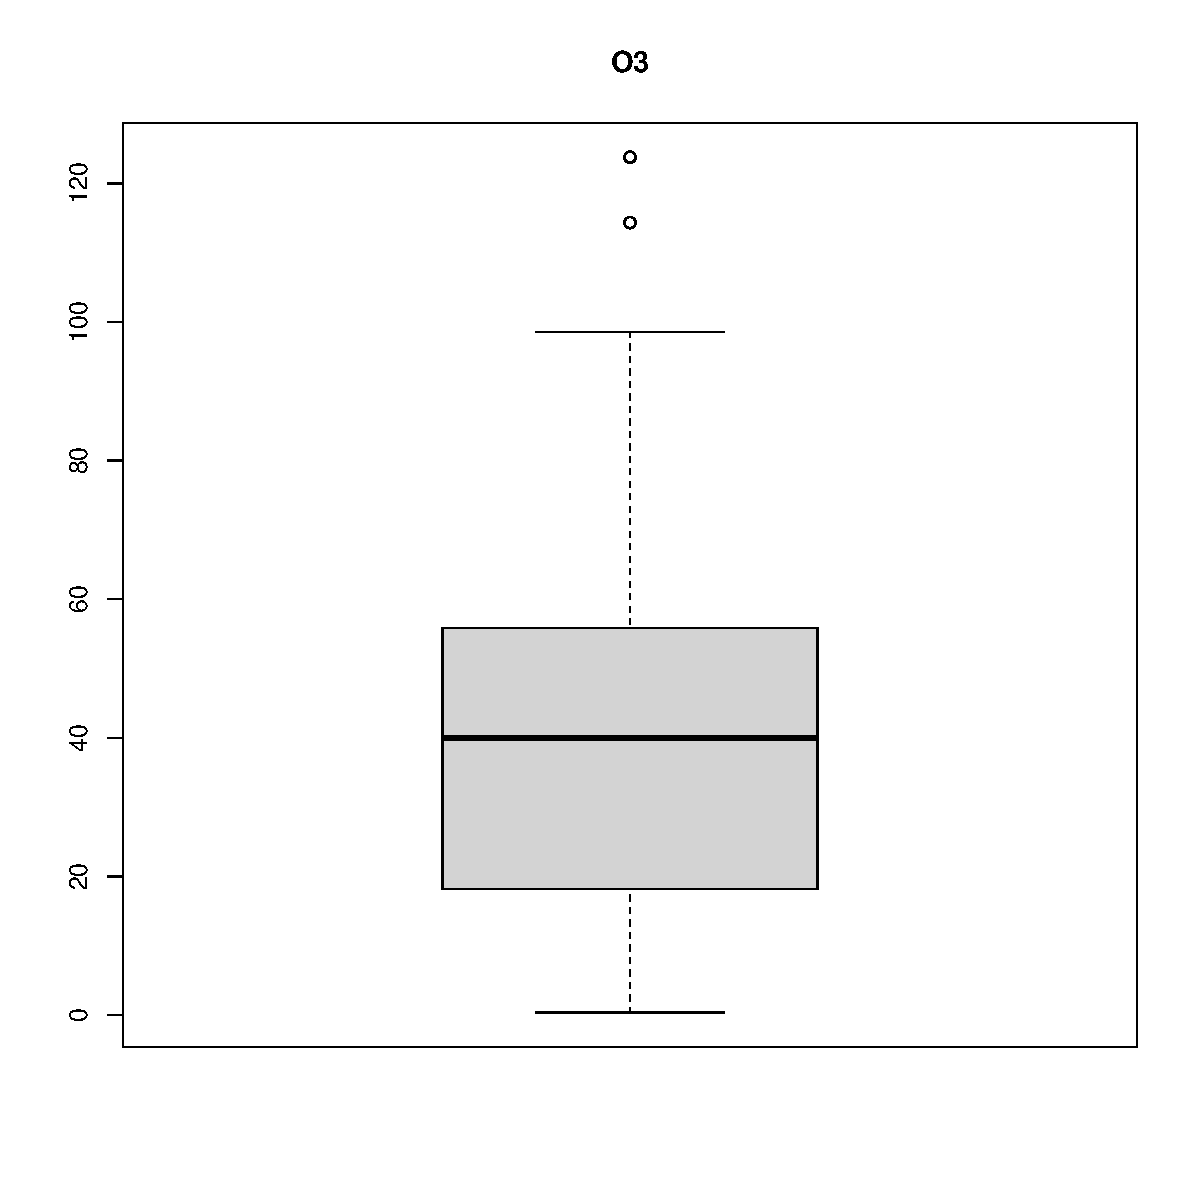
\includegraphics[width=0.4\linewidth]{figures/O3_box.pdf}
    \caption{boxplot}
\end{figure}
Observing the boxplot of PM2.5, it is obvious that the median corresponding to the middle line of the box is 6.3, which means that the concentration of 6.3 is the average level of PM2.5 pollutants, and the upper and lower limits of the box represent one fourth and three fourth of the value of concentration of PM2.5 in the data set. This shows that the concentration of PM2.5 pollutants mostly fluctuates from 7.1 to 5.9. There are two lines above and below the box representing the maximum value of 9.43 and the minimum value of 5.09, and there are five points above the maximum line that are out of range. These five points are outliers.
\\
\\
Observing the boxplot of NO2, you will find that the median corresponding to the middle line of the box is 44, which means that the concentration of 44 reflects the average level of NO2 pollutants, and the upper and lower limits of the box represent the upper four-digit fraction of NO2 respectively. and the next four digits. This shows that the concentration of NO2 pollutants mostly fluctuates from 31 to 66. There are two lines above and below the box representing the maximum value of 114.65 and the minimum value of 5.97, and there are three points above the maximum line that are out of range. These three points are outliers.
\\
\\
Observing the boxplot of O3, you will find that the median corresponding to a line in the middle of the box is 40, then it can be shown that the concentration of 40 reflects the average level of O3 pollutants, and the upper and lower limits of the box represent the O3. Upper four-digit score and lower four-digit score. This shows that the concentration of O3 pollutants mostly fluctuates from 18 to 56. There are two lines above and below the box representing the maximum value of 98.52 and the minimum value of 0.35. There are two points above the maximum line that are out of range, which are outliers.

% \cite{Linear}
% \subsection{NO2}
% \begin{figure}[H]
%     \centering
%     \vspace{-0.35cm}
%     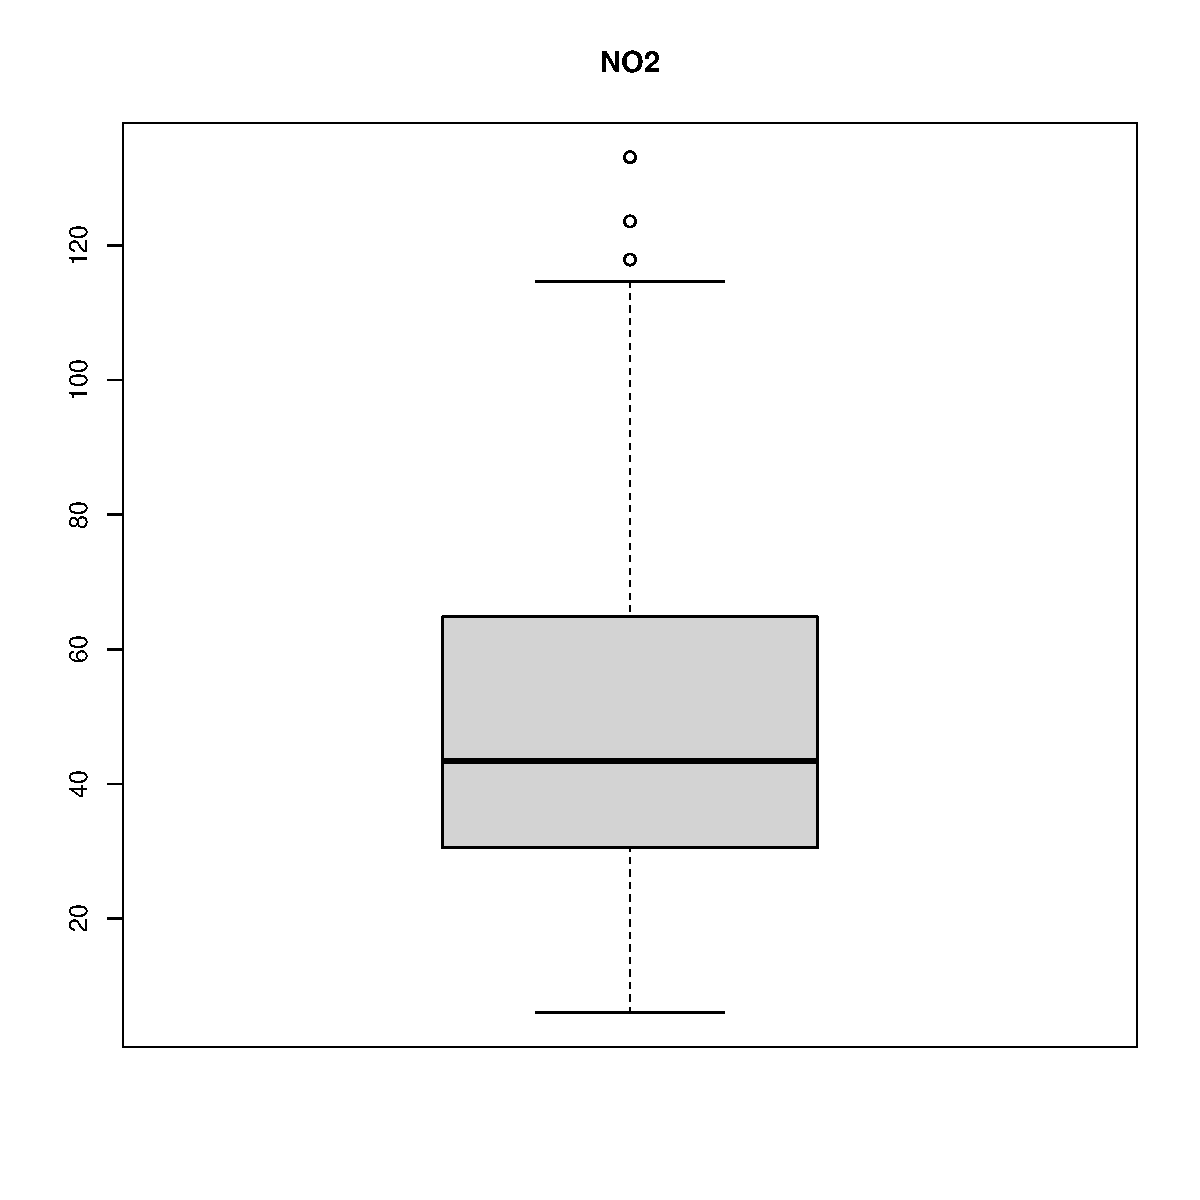
\includegraphics[width=0.7\linewidth]{figures/NO2_box.pdf}
%     \caption{NO2 box}
% \end{figure}
% \subsection{O3}
% \begin{figure}[H]
%     \centering
%     \vspace{-0.35cm}
%     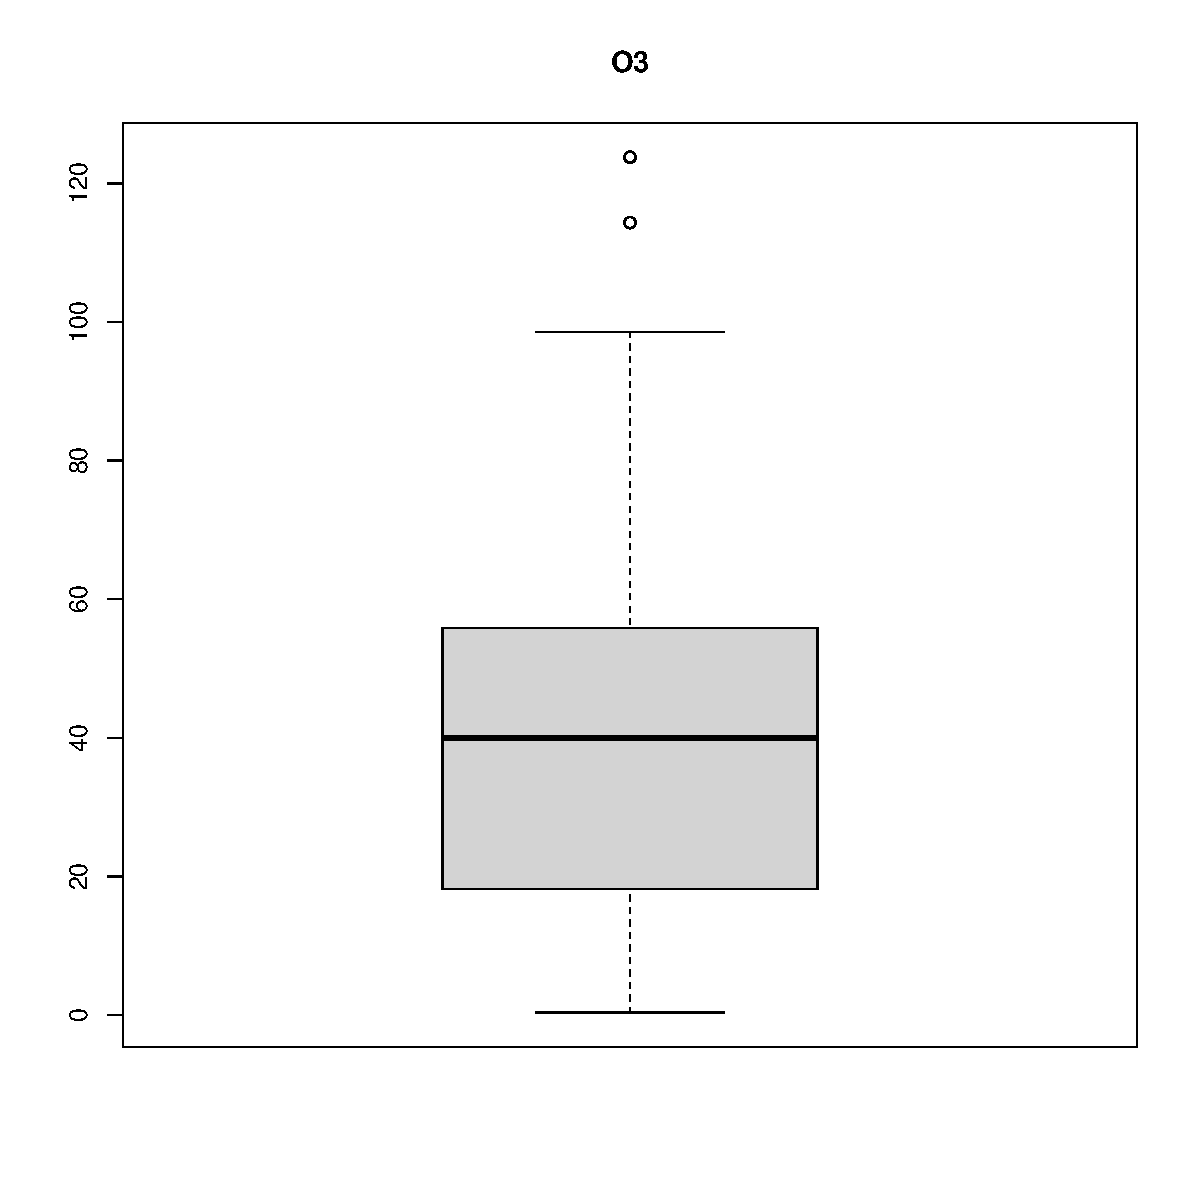
\includegraphics[width=0.7\linewidth]{figures/O3_box.pdf}
%     \caption{O3 box}
% \end{figure}

% --------------------------------------------------------
% Section 3: more advanced statistics
% --------------------------------------------------------
\section{more advanced statistics}
\label{sec:more advanced statistics}
\begin{figure}[H]
    \centering
    \vspace{-0.35cm}
    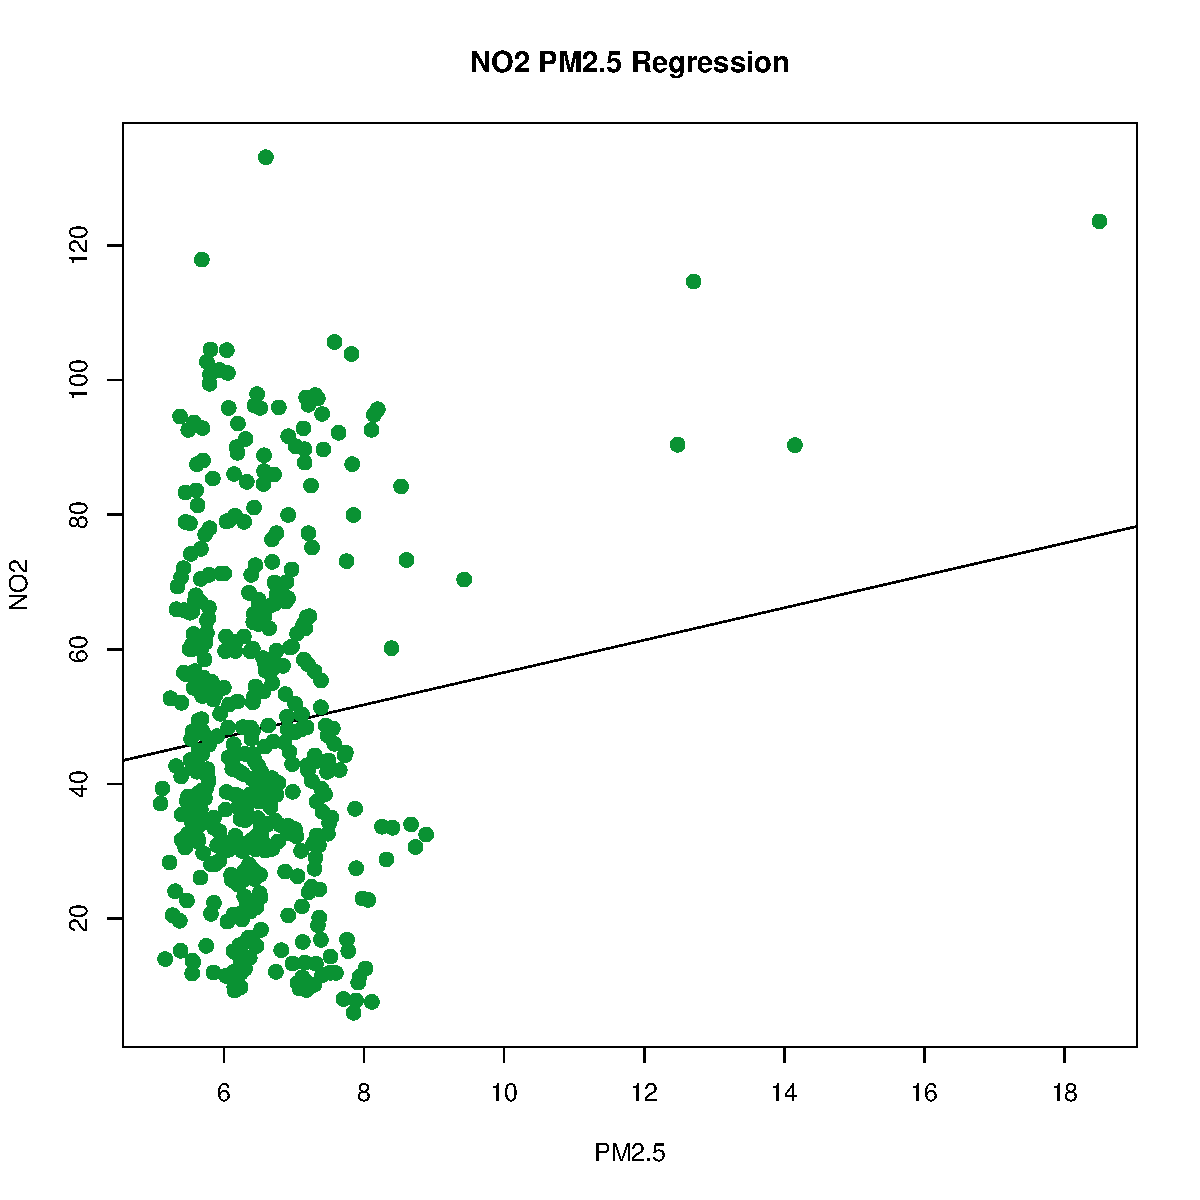
\includegraphics[width=0.4\linewidth]{figures/NO2_PM25_Regression.pdf}
    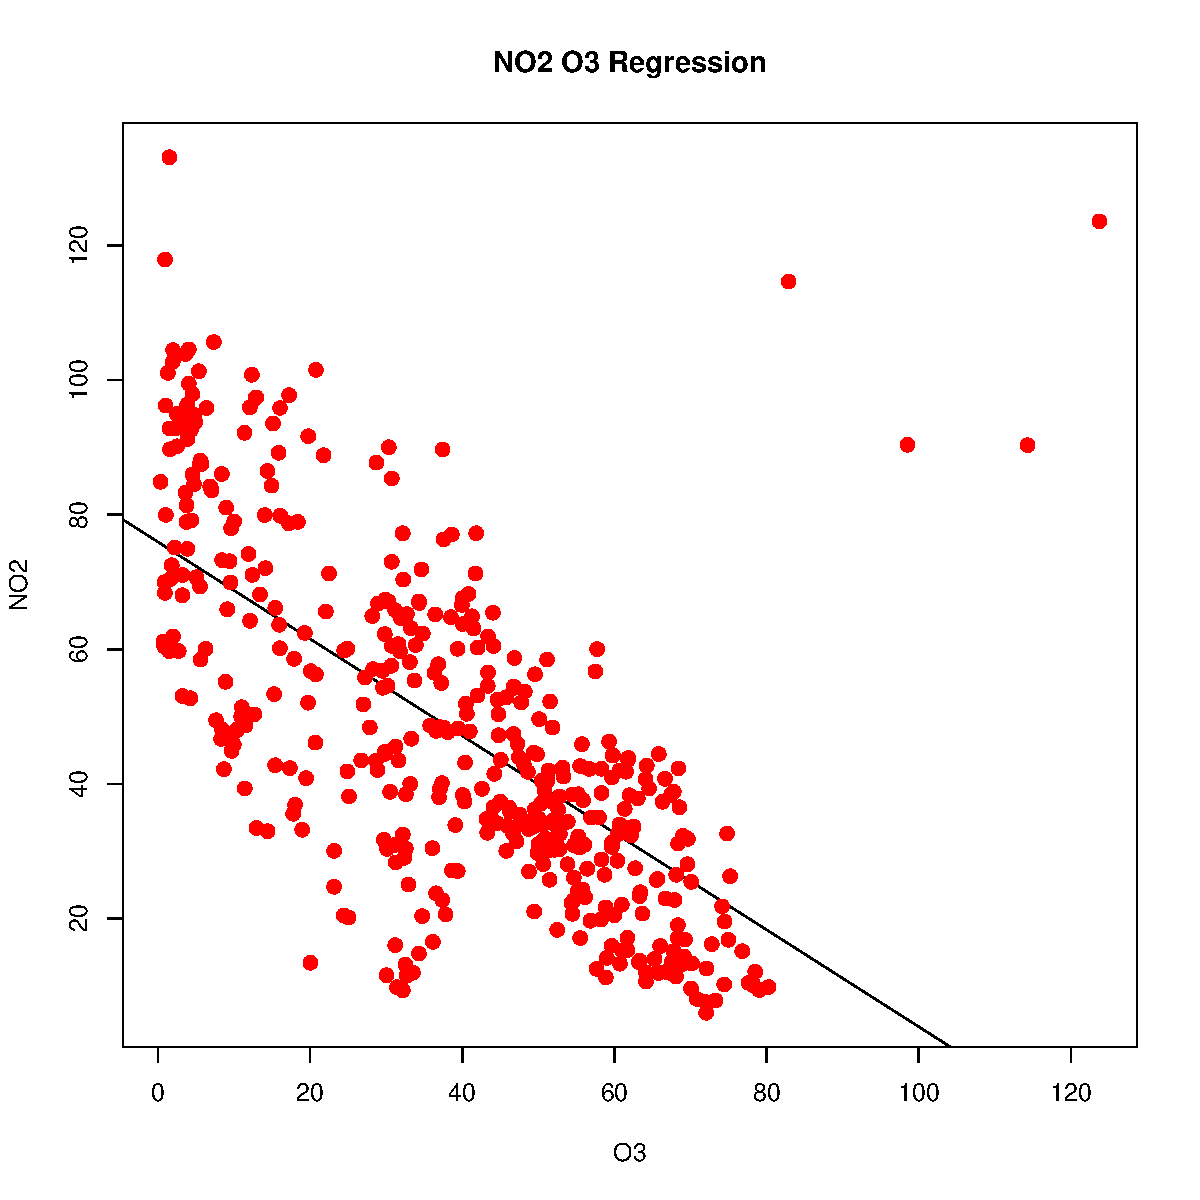
\includegraphics[width=0.4\linewidth]{figures/NO2_O3_Regression.pdf}
    % \caption{}
\end{figure}
The plots show a negative trend between NO2 and O3. While the trend is less clear between NO2 and PM2.5, there is a slight positive association.
That is, more O3 is associated with a lower NO2, and higher PM2.5 is associated with a higher NO2.
\\
We can use ``cor'' command in R to calculate the correlation with two variables below:
\begin{lstlisting}
    > cor(data$NO2, data$PM2.5)
    [1] 0.1036955
    > cor(data$NO2, data$O3)   
    [1] -0.6475529
\end{lstlisting}
The calculation results show the same conclusion as the image, 
the correlation between NO2 and PM2.5 is only 0.1036955 which means a slight positive association, 
and the correlation between NO2 and O3 is -0.6475529 which shows there is a negative trend.
\\
We have the formula
\begin{equation}
    R^2=1-\frac{SSE}{SST}
\end{equation}
By using ``summary'' command in R, we can get the value of $R^2$ to show the predict model good or not.
We denote the modoel NO2 $\sim$ O3 with model1 and the modoel NO2 $\sim$ PM2.5 with model2, and a predict model is built by ``lm'' command in R:
\begin{lstlisting}
    > model1 = lm(NO2 ~ O3, data=data)
    > summary(model1)

    Call:
    lm(formula = NO2 ~ O3, data = data)
    ... ...
    Multiple R-squared:  0.4193,    Adjusted R-squared:  0.418

    > model2 = lm(NO2 ~ PM2.5, data=data)
    > summary(model2)

    Call:
    lm(formula = NO2 ~ PM2.5, data = data)
    ... ...
    Multiple R-squared:  0.01075,   Adjusted R-squared:  0.008554 
\end{lstlisting}
These show that the $R^2$ of model1 is 0.4193, and the $R^2$ of model2 is 0.01075 which means model1 is much better than model2.
% --------------------------------------------------------
% Section 4: multi variable regression forecasting models, visualisation of results
% --------------------------------------------------------
\section{multi variable regression forecasting models, visualisation of results}
\label{sec:multi variable regression forecasting models, visualisation of results}
We denote the model NO2 $\sim$ O3 + PM2.5 with model3, and build a predict model by ``lm'' command in R and show the results by ``summary'' command:
\begin{lstlisting}
    > model3 = lm(NO2 ~ O3 + PM2.5, data=data)
    > summary(model3)

    Call:
    lm(formula = NO2 ~ O3 + PM2.5, data = data)

    Residuals:
        Min      1Q  Median      3Q     Max
    -54.701 -11.939  -0.712  12.328  56.725

    Coefficients:
                Estimate Std. Error t value Pr(>|t|)
    (Intercept) 30.72543    5.04722   6.088 2.46e-09 ***
    O3          -0.82857    0.03827 -21.649  < 2e-16 ***
    PM2.5        7.54685    0.79694   9.470  < 2e-16 ***
    ---
    Signif. codes:  0 '***' 0.001 '**' 0.01 '*' 0.05 '.' 0.1 ' ' 1

    Residual standard error: 17.7 on 449 degrees of freedom
    Multiple R-squared:  0.516,     Adjusted R-squared:  0.5138
    F-statistic: 239.3 on 2 and 449 DF,  p-value: < 2.2e-16
\end{lstlisting}




% --------------------------------------------------------
% Section 5: model performance and discussion of results
% --------------------------------------------------------
\section{model performance and discussion of results}
\label{sec:model performance and discussion of results}

The results show that the $R^2$ of model3 is 0.516 which is larger than the model1 and model2. Also, the adjusted R-squared shows the same results.
From code in section 4, line 17, the number of stars represent the significance of the group of data to the model.
And the stars of O3 and PM2.5 both are three stars which means they both are very significant to this model.
The prediction performance could be improved by using multi variable regression forecasting model. For the current model, several ways could be chosen to improve accuracy of the prediction. For example adding temperature and humidity data to linear regression could be a possible option to optimize the model. 
Moreover, adding different weights to various variables is also a good way to optimize the model.


% --------------------------------------------------------
% Section 6: Conclusions
% --------------------------------------------------------
\section{Conclusions}
    In conclusion, the analysis and comparison of the NO2, O3 and PM2.5 data by using R show that NO2 is positively associated with PM2.5 and negatively associated with O3. The $R^2$ of the multivariate regression model is closer to 1 than that of the single-variable regression model when both PM2.5 and O3 are used as independent variables of NO2. Hence, the regression equation fitted by the multivariate regression model is better than the single-variable regression equation, and its performance is also better, and the final forecasting results are more accurate by using multivariate regression. Several options that could improve better results are mentioned above and the combination of them with multivariate regression could produce more accurate forecasting trend of data.



\bibliographystyle{IEEEtran}
\bibliography{References}

\end{document}